
\documentclass[mathserif]{beamer}
\usepackage{stmaryrd}
\usepackage{semantic}
\usepackage{listings}
\usepackage{algorithmicx}
\usepackage{mathtools}

%\usetheme{Madrid}
\usetheme{Luebeck}
%\usecolortheme{mmv}
% Uncomment the following line if you want %
% page numbers and using Warsaw theme%
\setbeamertemplate{footline}[frame number]
\setbeamercovered{transparent}

\setbeamercovered{invisible}
% To remove the navigation symbols from1
% the bottom of slides%
\setbeamertemplate{navigation symbols}{} 
\setbeamerfont{mathserif}{size=\footnotesize}
\newcommand{\updt}[1]{{\color{blue}#1}}

\usepackage{graphicx}
%\usepackage{bm}         % For typesetting bold math (not \mathbold)
%\logo{\includegraphics[height=0.6cm]{CU_logo.png}}

\title[Gradual Python]{Reticulated Python\\
and Gradual Typing with Assertions}
\author[Vitousek, Siek]
       {\textcolor{blue}{Michael M. Vitousek}\and Jeremy G. Siek}
\date{\today}

\newcommand{\of}{{:}}
\newcommand{\dyn}{{?}}
\newcommand{\Dyn}{\textsf{Dyn}}

\newcommand{\ite}[3]{\mathsf{if}\, #1 \,\mathsf{then}\, #2 \,\mathsf{else}\, #3}
\newcommand{\inserts}{\Longrightarrow}
\newcommand{\cast}[2]{(#1)#2}
\newcommand{\Gbox}[1]{\colorbox{lightgray}{\ensuremath{#1}}}
\newcommand{\Rbox}[1]{\colorbox{red}{\ensuremath{#1}}}
\newcommand{\threesome}[3]{#1\xRightarrow{#2} #3}
%\newcommand{\pif}{}
\newcommand{\pif}{}

\lstset{ %
  language=python,                % the language of the code
  showspaces=false,               % show spaces adding particular underscores
  showstringspaces=false,         % underline spaces within strings
  showtabs=false,                 % show tabs within strings adding particular underscores
  tabsize=2,                      % sets default tabsize to 2 spaces
  captionpos=b,                   % sets the caption-position to bottom
  breaklines=true,                % sets automatic line breaking
  breakatwhitespace=false,        % sets if automatic breaks should only happen at whitespace
  escapeinside={\%*}{*)},         % if you want to add a comment within your code
  mathescape,
  %morekeywords={*,...}           % if you want to add more keywords to the set
}

\begin{document}
%
\begin{frame}
\titlepage
\end{frame}
%

\section{Introduction}
\begin{frame}{Introduction}
  \begin{itemize}
  \item Gradual typing in Python
    \begin{itemize}
    \item Compile-time error detection 
    \item Blame tracking 
    \item More efficient programs\pif
    \end{itemize}
  \item Several different schemes
    \begin{itemize}
    \item Casts on complex values
    \end{itemize}
  \item Want to be able to prototype these approaches,
  \item and be able to actually run code
  \end{itemize}
\end{frame}

\begin{frame}{Setting}
  \begin{itemize}
  \item Gradual Jython
    \begin{itemize}
    \item Very promising optimization results (see Shashank's thesis)
    \item Not especially agile
    \end{itemize}
  \item Come back to this when we know more, but for now...
  \end{itemize}
\end{frame}
\section{Reticulated Python}
\begin{frame}{RETICULATED PYTHON}
  \begin{center}
    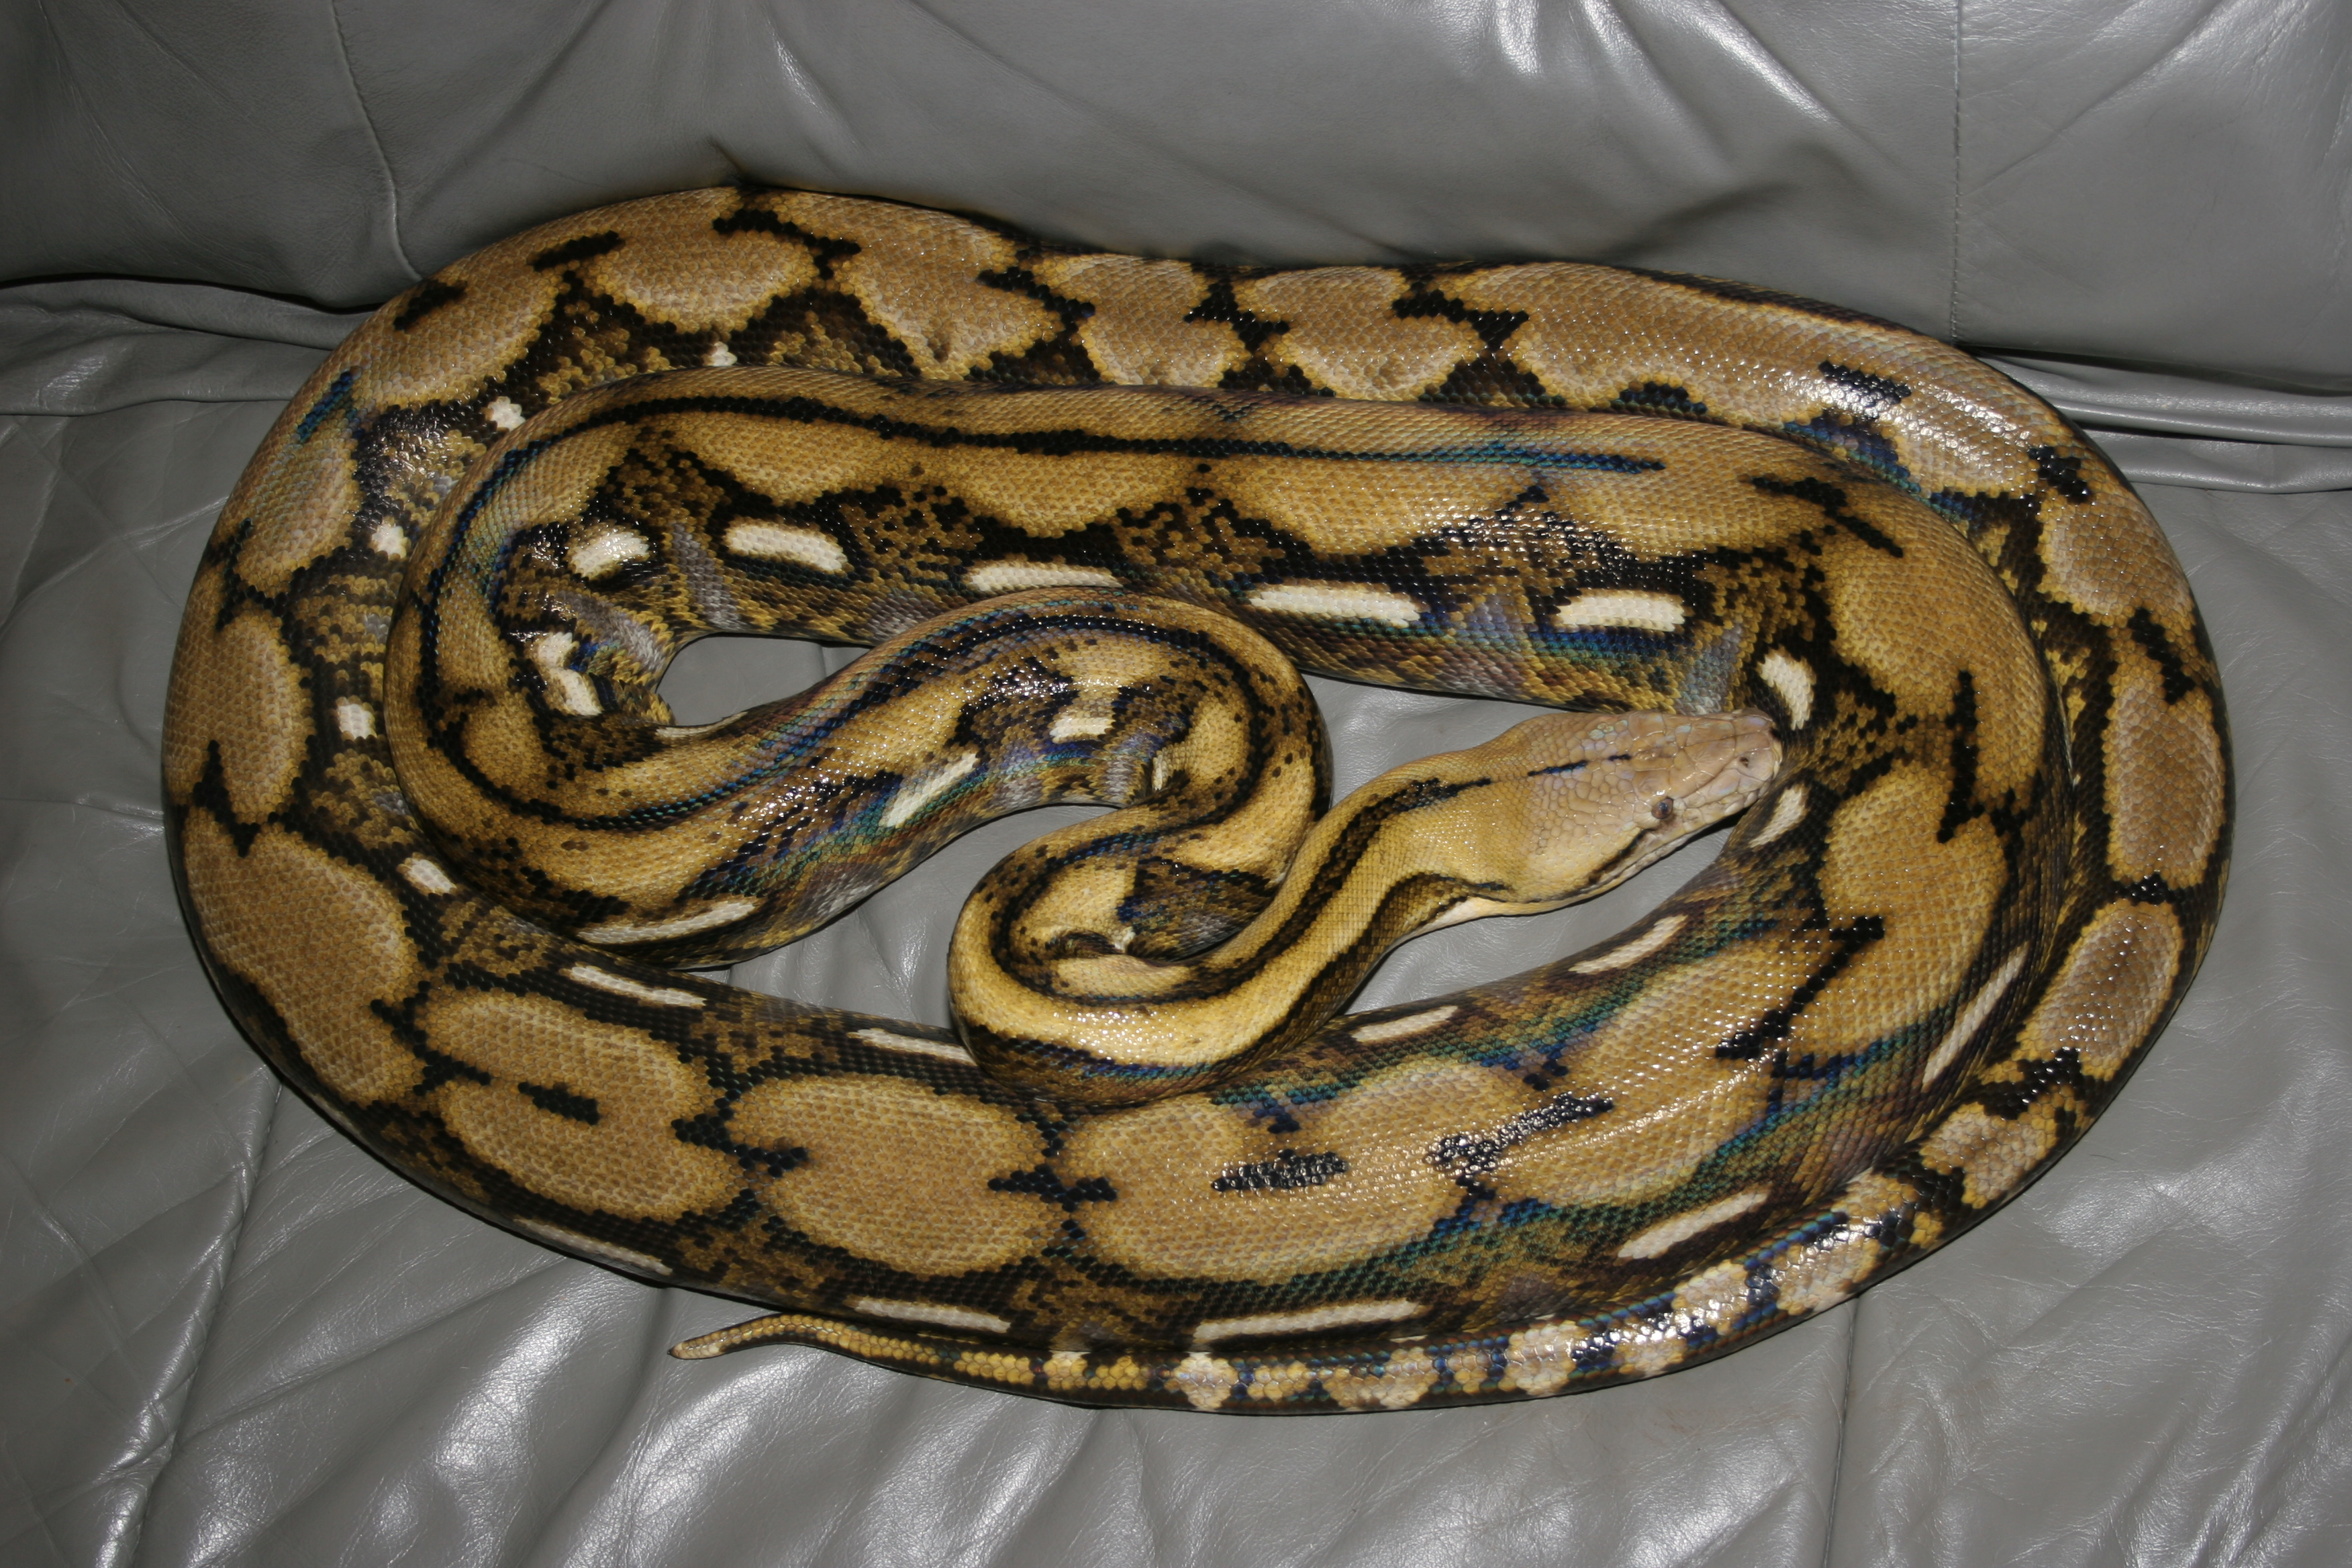
\includegraphics[scale=.08]{Reticulated_python_MP1.JPG}  
  \end{center}
\end{frame}

\begin{frame}{Reticulated Python}
  \begin{itemize}
  \item Lightweight gradual typing for Python 3
    \begin{itemize}
    \item Easy prototyping of gradual typing schemes
    \item Straightforward to use --- \texttt{retic.py myTypedModule.py}
    \item Not concerned with optimization
    \end{itemize}
  \item Two parts
    \begin{itemize}
    \item Source-to-source transformer: typechecking and cast insertion
    \item Runtime library to support casts
    \end{itemize}
  \end{itemize}
\end{frame}

\begin{frame}{Typechecking}
 \begin{algorithmic}[2]
    \State def m(x:bool, f:Function(int,int))$\to$int:
    \State \;\;\;return f(x)
    \State 
    \State m(True, $\lambda$ x. x)
  \end{algorithmic}
\end{frame}

\addtocounter{framenumber}{-1}
\begin{frame}{Typechecking}
 \begin{algorithmic}[2]
    \State def m(x:bool, f:Function(int,int))$\to$int:
    \State \;\;\;return {\color{red}f(x)}
    \State 
    \State m(True, $\lambda$ x. x)
  \end{algorithmic}
\end{frame}

\begin{frame}{Cast insertion}
 \begin{algorithmic}[2]
    \State def m(x, f:Function(int,int))$\to$int:
    \State \;\;\;return f(x)
    \State 
    \State m(True, $\lambda$ x. x)
    \State
  \end{algorithmic}
\end{frame}

\addtocounter{framenumber}{-1}
\begin{frame}{Cast insertion}
 \begin{algorithmic}[2]
    \State def m(x, f:Function(int,int))$\to$int:
    \State \;\;\;return f({\color{blue}cast(}x{\color{blue},Dyn,int)})
    \State 
    \State m({\color{blue}cast(}True{\color{blue},bool,Dyn)}, 
    \State \;\;{\color{blue}cast(}$\lambda$ x. x{\color{blue},Function(Dyn,Dyn),Function(int,int)})
  \end{algorithmic}
\end{frame}

\begin{frame}{Cast insertion}
  \begin{itemize}
  \item AST is Python3 valid before and after cast insertion
  \item Definition of \textit{cast} provided at runtime
    \begin{itemize}
    \item Choice of this definition specifies what implementation scheme we're using
    \end{itemize}
  \end{itemize}
\end{frame}

\section{Casts-as-Assertions}
\begin{frame}{Casts}
  \begin{itemize}
  \item Casts on basic values
    \begin{itemize}
    \item Just asserts
    \item Maybe with boxing/unboxing
    \end{itemize}
  \item Functions, other complex values harder
  \end{itemize}
  \begin{center}
    cast($\lambda$ x. x, Function(Dyn,Dyn), Function(Int,Int))$\equiv$\\
    $\lambda$ y:Int. cast(($\lambda$ x. x)(cast(y,Int,Dyn)), Dyn, Int)
  \end{center}
  \begin{itemize}
  \item Better ways of doing this
    \begin{itemize}
    \item Still need to wrap or attach cast info to function at runtime 
    \end{itemize}
  \end{itemize}
\end{frame}

\begin{frame}{Casts-as-assertions}
  \begin{itemize}
  \item Can we have gradual typing without runtime modification of values/only using asserts?
  \item Cast-as-assertion model:
    \begin{itemize}
    \item All casts are assertions, which shallowly check the type of a value
    \item Can never trust deeper type info without checks
    \end{itemize}
  \item More compile-time checks need to be inserted to check that values correspond to locally expected type
  \end{itemize}
\end{frame}

\begin{frame}{Cast insertion}
 \begin{algorithmic}[2]
    \State def m(x, f:Function(int,int))$\to$int:
    \State \;\;\;return f({\color{blue}cast(}x{\color{blue},Dyn,int)})
    \State 
    \State m({\color{blue}cast(}True{\color{blue},bool,Dyn)}, 
    \State \;\;{\color{blue}cast(}$\lambda$ x. x{\color{blue},Function(Dyn,Dyn),Function(int,int)})
  \end{algorithmic}
\end{frame}

\addtocounter{framenumber}{-1}
\begin{frame}{Cast insertion}
 \begin{algorithmic}[2]
    \State def m(x, f:Function(int,int))$\to$int:
    \State \;\;\;return check(f({\color{blue}cast(}x{\color{blue},Dyn,int)}), int)
    \State 
    \State check(m({\color{blue}cast(}True{\color{blue},bool,Dyn)}, 
    \State \;\;{\color{blue}cast(}$\lambda$ x. x{\color{blue},Function(Dyn,Dyn),Function(int,int)}), int)
  \end{algorithmic}
\end{frame}

\addtocounter{framenumber}{-1}
\begin{frame}{Cast insertion}
 \begin{algorithmic}[2]
    \State def m(x, f:Function(int,int))$\to$int:
    \State \;\;\;check(f, Function(int, int))
    \State \;\;\;return check(f({\color{blue}cast(}x{\color{blue},Dyn,int)}), int)
    \State 
    \State check(m({\color{blue}cast(}True{\color{blue},bool,Dyn)}, 
    \State \;\;{\color{blue}cast(}$\lambda$ x. x{\color{blue},Function(Dyn,Dyn),Function(int,int)}), int)
  \end{algorithmic}
\end{frame}

\begin{frame}{Forgotten history}
  \begin{itemize}
  \item This allows functions to go through casts like
\[\Dyn\to \Dyn \Rightarrow Int \to Int \Rightarrow \Dyn \to \Dyn \Rightarrow \]\[Bool \to Bool\Rightarrow \Dyn\to \Dyn\]
\item Blah
  \end{itemize}
\end{frame}
\end{document}
\begin{frame}{Aims}
  \begin{itemize}
  \item Preserve type safety\pause
  \item Make it fast\pause
  \item Track blame\pause
  \item Correspond with Java object model
  \end{itemize}
\end{frame}

\section{Kinds of casts}
\subsection{Casts-as-assertions}
\begin{frame}{Casts-as-assertions}\pause
  \begin{itemize}
  \item Casts on objects are only checks\pause
  \item No mutation or further checking\pause
  \end{itemize}
 \begin{algorithmic}[1]
    \State $\textit{obj1}\of\{\textit{x}\of\star, \textit{y}\of\star\}=\{\textit{x} = 10{::}\threesome{\mathsf{int}}{}{\star}, \textit{y} = \mathsf{True}{::}\threesome{\mathsf{bool}}{}{\star}\}$
    \State $\textit{obj2}\of\{\textit{x}\of\mathsf{int}, \textit{y}\of\mathsf{bool}\}=\textit{obj1}{::}\threesome{\{\textit{x}\of\star, \textit{y}\of\star\}}{}{\{\textit{x}\of\mathsf{int}, \textit{y}\of\mathsf{bool}\}}$
    \State $\textit{obj1}.\textit{x}=\text{``Hello world''}{::}\threesome{\mathsf{str}}{}{\star}$
    \State \textit{print obj2.x}
  \end{algorithmic}\pause
  \begin{itemize}
  \item Program is fine as is\pause
  \item \textit{obj2.x} is typed $\star$
  \end{itemize}
\end{frame}

\begin{frame}{Casts-as-assertions}
  \begin{itemize}
  \item Cons\pause
    \begin{itemize}
    \item Terrible \pause(as an implementation of GT)\pause
    \end{itemize}
  \item Pros
    \begin{itemize}
    \item Easy to implement \pause
    \item Syntactic transformation on current Python
    \end{itemize}
  \end{itemize}
\end{frame}

\subsection{Transient casts}
\begin{frame}{Transient casts}
  \begin{itemize}
  \item Casts on objects create proxies\pause
  \item Reads via proxies have casts applied\pause
  \end{itemize}
 \begin{algorithmic}[1]
    \State $\textit{obj1}\of\{\textit{x}\of\star, \textit{y}\of\star\}=\{\textit{x} = 10{::}\threesome{\mathsf{int}}{}{\star}, \textit{y} = \mathsf{True}{::}\threesome{\mathsf{bool}}{}{\star}\}$
    \State $\textit{obj2}\of\{\textit{x}\of\mathsf{int}, \textit{y}\of\mathsf{bool}\}=\textit{obj1}{::}\threesome{\{\textit{x}\of\star, \textit{y}\of\star\}}{}{\{\textit{x}\of\mathsf{int}, \textit{y}\of\mathsf{bool}\}}$
    \State $\textit{obj1}.\textit{x}=\text{``Hello world''}{::}\threesome{\mathsf{str}}{}{\star}$
    \State \textit{print {\color{red}obj2.x}}\pause
  \end{algorithmic}
  \begin{itemize}
  \item \textit{obj2.x} has cast $\threesome{\star}{}{\textsf{int}}$ applied at runtime when read
  \end{itemize}
\end{frame}

\begin{frame}{Transient casts}
  \begin{itemize}
  \item Pros
    \begin{itemize}
    \item Flexible, ``Pythonic''\pause
    \end{itemize}
  \item Cons
    \begin{itemize}
    \item Requires casts to be applied at every read
    \end{itemize}
  \end{itemize}
\end{frame}

\subsection{Monotonic casts}
\begin{frame}{Monotonic casts}
  \begin{itemize}
  \item Object casts \textit{permanently} alter the internal type of an object\pause
  \item Written values are cast to the current internal type of the object\pause
  \item Reads are either just upcasts, or are direct memory accesses\pause
  \end{itemize}
 \begin{algorithmic}[1]
    \State $\textit{obj1}\of\{\textit{x}\of\star, \textit{y}\of\star\}=\{\textit{x} = 10{::}\threesome{\mathsf{int}}{}{\star}, \textit{y} = \mathsf{True}{::}\threesome{\mathsf{bool}}{}{\star}\}$
    \State $\textit{obj2}\of\{\textit{x}\of\mathsf{int}, \textit{y}\of\mathsf{bool}\}=\textit{obj1}{::}\threesome{\{\textit{x}\of\star, \textit{y}\of\star\}}{}{\{\textit{x}\of\mathsf{int}, \textit{y}\of\mathsf{bool}\}}$
    \State ${\color{red}\textit{obj1}.\textit{x}=\text{``Hello world''}{::}\threesome{\mathsf{str}}{}{\star}}$
    \State \textit{print obj2.x}
  \end{algorithmic}\pause
  \begin{itemize}
  \item $(\text{``Hello world''}{::}\threesome{\mathsf{str}}{}{\star})$ is
    cast by $\threesome{\star}{}{\mathsf{int}}$
  \end{itemize}
\end{frame}

\begin{frame}{Monotonic casts}
  \begin{itemize}
  \item Pros
    \begin{itemize}
    \item Fast, unboxed reads from typed objects\pause
    \item Safe upcasts only on reads from untyped objects\pause
    \item Reads always succeed\pause
    \item Underlying object always consistent with all types it has been referenced by\pause
    \end{itemize}
  \item Cons
    \begin{itemize}
    \item Action at a distance\pause
    \item Types persist after reference leaves scope
    \end{itemize}
  \end{itemize}
\end{frame}

\begin{frame}{Other approaches}
  \begin{itemize}
  \item Scoped monotonic casts
    \begin{itemize}
    \item Casts are monotonic within a certain range
    \item Alleviates some action-at-a-distance issues, still an issue with concurrency\pause
    \end{itemize}
  \item Monotonic casts with transient fallback
    \begin{itemize}
    \item Implementation of transient casts
    \item Works as monotonic until conflict, then transient
    \end{itemize}
  \end{itemize}
\end{frame}

\section{Monotonic casts}
\begin{frame}{Static and memory types at cast site}
 \begin{algorithmic}[1]
    \State $\textit{obj1}\of\{\textit{x}\of\star, \textit{y}\of\star\}=\{\textit{x} = 10{::}\threesome{\mathsf{int}}{}{\star}, \textit{y} = \mathsf{True}{::}\threesome{\mathsf{bool}}{}{\star}\}$
    \State $\textit{obj2}\of\{\textit{x}\of\star, \textit{y}\of\mathsf{bool}\}=\textit{obj1}{::}\threesome{\{\textit{x}\of\star, \textit{y}\of\star\}}{}{\{\textit{x}\of\star, \textit{y}\of\mathsf{bool}\}}$
    \State $\textit{obj3}\of\{\textit{x}\of\mathsf{int}, \textit{y}\of\mathsf{bool}\}=\textit{obj1}{::}\threesome{\{\textit{x}\of\star, \textit{y}\of\star\}}{}{\{\textit{x}\of\mathsf{int}, \textit{y}\of\mathsf{bool}\}}$
  \end{algorithmic}
  \begin{itemize}
  \item At line 3:\pause
    \begin{itemize}
    \item Cast source type: $\{x\of\star, y\of\star\}$\pause
    \item Cast target type: $\{x\of\mathsf{int}, y\of\mathsf{bool}\}$\pause
    \item Actual runtime type before cast: $\{x\of\star, y\of\mathsf{bool}\}$
    \end{itemize}\pause
  \item Actual cast: $\threesome{\{x\of\star, y\of\mathsf{bool}\}}{}{\{x\of\mathsf{int}, y\of\mathsf{bool}\}}$\pause
  \item More complex: blame labels, threesome labeled types, memory labeled types
  \end{itemize}
\end{frame}

\begin{frame}{Monotonic reads} 
\begin{algorithmic}[1]
    \State $\textit{obj1}\of\{\textit{x}\of\star, \textit{y}\of\star\}=\{\textit{x} = 10{::}\threesome{\mathsf{int}}{}{\star}, \textit{y} = \mathsf{True}{::}\threesome{\mathsf{bool}}{}{\star}\}$
    \State $\textit{obj2}\of\{\textit{x}\of\mathsf{int}, \textit{y}\of\mathsf{bool}\}=\textit{obj1}{::}\threesome{\{\textit{x}\of\star, \textit{y}\of\star\}}{}{\{\textit{x}\of\mathsf{int}, \textit{y}\of\mathsf{bool}\}}$
    \State \textit{obj2.x}
    \State \textit{obj1.x}
  \end{algorithmic}
  
  \begin{itemize}
  \item[] \color{white} Direct accesses are distinguished syntactically (during cast insertion)
  \item[] Indirect accesses have static type syntactically added
    \begin{itemize}
    \item[]\color{white} At read, \textit{obj1.x} cast by $\threesome{\mathsf{int}}{}{\star}$
    \end{itemize}
  \end{itemize}
\end{frame}

\begin{frame}{Monotonic reads} 
  \addtocounter{framenumber}{-1}
  \begin{algorithmic}[1]
    \State $\textit{obj1}\of\{\textit{x}\of\star, \textit{y}\of\star\}=\{\textit{x} = 10{::}\threesome{\mathsf{int}}{}{\star}, \textit{y} = \mathsf{True}{::}\threesome{\mathsf{bool}}{}{\star}\}$
    \State $\textit{obj2}\of\{\textit{x}\of\mathsf{int}, \textit{y}\of\mathsf{bool}\}=\textit{obj1}{::}\threesome{\{\textit{x}\of\star, \textit{y}\of\star\}}{}{\{\textit{x}\of\mathsf{int}, \textit{y}\of\mathsf{bool}\}}$
    \State \textit{obj2[x]} \# Direct access
    \State \textit{obj1.x} 
  \end{algorithmic}
  \begin{itemize}
  \item Direct accesses are distinguished syntactically (during cast insertion)
  \item[]\color{white} Indirect accesses have static type syntactically added
    \begin{itemize}
    \item[]\color{white} At read, \textit{obj1.x} cast by $\threesome{\mathsf{int}}{}{\star}$
    \end{itemize}
  \end{itemize}
\end{frame}

\begin{frame}{Monotonic reads} 
  \addtocounter{framenumber}{-1}
  \begin{algorithmic}[1]
    \State $\textit{obj1}\of\{\textit{x}\of\star, \textit{y}\of\star\}=\{\textit{x} = 10{::}\threesome{\mathsf{int}}{}{\star}, \textit{y} = \mathsf{True}{::}\threesome{\mathsf{bool}}{}{\star}\}$
    \State $\textit{obj2}\of\{\textit{x}\of\mathsf{int}, \textit{y}\of\mathsf{bool}\}=\textit{obj1}{::}\threesome{\{\textit{x}\of\star, \textit{y}\of\star\}}{}{\{\textit{x}\of\mathsf{int}, \textit{y}\of\mathsf{bool}\}}$
    \State \textit{obj2[x]} \# Direct access
    \State \textit{obj1.(x~$:\star$)} \# Indirect access
  \end{algorithmic}
  \begin{itemize}
  \item Direct accesses are distinguished syntactically (during cast insertion)
  \item Indirect accesses have static type syntactically added\pause
    \begin{itemize}
    \item At read, \textit{obj1.x} cast by $\threesome{\mathsf{int}}{}{\star}$
    \end{itemize}
  \end{itemize}
\end{frame}

\end{document}




















\begin{frame}{Outline}
\tableofcontents
\end{frame}

\AtBeginSection[]
{
  \begin{frame}{Outline}
    \tableofcontents[currentsection]
  \end{frame}
} 

\section{Function casts}
\subsection{Motivation}

\begin{frame}{Function casts: motivation and example}

  \begin{algorithmic}[1]
  \State \textbf{def} $\textit{explore\_files}(\textit{files}, \textit{fun})\of$
  \State \;\;\;\textbf{for} $\textit{file}\textbf{ in }\textit{files}\of$
  \State \;\;\;\;\;\;\textbf{if} $\textit{file}.\textit{is\_directory}()\of$
  \State \;\;\;\;\;\;\;\;\;$\textit{explore\_dir}(\textit{file}{\color{white} : \dyn \Rightarrow \mathsf{file}}, \textit{fun}{\color{white} : \dyn \Rightarrow \mathsf{file}\to\mathsf{str}})$
  \State \;\;\;\;\;\;\textbf{else}\of \textbf{ print} $\textit{fun}(\textit{file})$
  \State \textbf{def} $\textit{explore\_dir}(\textit{dir}\of\mathsf{file}, \textit{fun}\of\mathsf{file}\to\mathsf{str}) \to \mathsf{unit}\of$
  \State \;\;\;$\textit{explore\_files}(\textit{file}.\textit{members}(){\color{white} : \mathsf{list} \Rightarrow \dyn}, \textit{fun}{\color{white} : \mathsf{file} \to \mathsf{str} \Rightarrow \dyn})$
  \vfill
  \begin{itemize}
  \item[] {\color{white} Standard gradual typing approach: inserted casts moderate
    between static and dynamic code}
    \begin{itemize}
    \item[] {\color{white} Simple for basic types (\texttt{int, float})}
    \item[] {\color{white} Harder for functions}
    \end{itemize}
  \end{itemize}
\end{algorithmic}
\end{frame}
\begin{frame}{Function casts: motivation and example}
  \addtocounter{framenumber}{-1}

  \begin{algorithmic}[1]
  \State \textbf{def} $\textit{explore\_files}(\textit{files}, \textit{fun})\of$
  \State \;\;\;\textbf{for} $\textit{file}\textbf{ in }\textit{files}\of$
  \State \;\;\;\;\;\;\textbf{if} $\textit{file}.\textit{is\_directory}()\of$
  \State \;\;\;\;\;\;\;\;\;$\textit{explore\_dir}(\textit{file}{\color{blue} : \dyn \Rightarrow \mathsf{file}}, \textit{fun}{\color{blue} : \dyn \Rightarrow \mathsf{file}\to\mathsf{str}})$
  \State \;\;\;\;\;\;\textbf{else}\of \textbf{ print} $\textit{fun}(\textit{file})$
  \State \textbf{def} $\textit{explore\_dir}(\textit{dir}\of\mathsf{file}, \textit{fun}\of\mathsf{file}\to\mathsf{str}) \to \mathsf{unit}\of$
  \State \;\;\;$\textit{explore\_files}(\textit{file}.\textit{members}(){\color{red} : \mathsf{list} \Rightarrow \dyn}, \textit{fun}{\color{red} : \mathsf{file} \to \mathsf{str} \Rightarrow \dyn})$
  \vfill
  \begin{itemize}
  \item Standard gradual typing approach: inserted casts moderate
    between static and dynamic code
    \begin{itemize}
    \item Simple for basic types (\texttt{int, float})
    \item Harder for functions
    \end{itemize}
  \end{itemize}
\end{algorithmic}
\end{frame}

\begin{frame}{Function casts induce overhead}
  \begin{itemize}
  \item Previous approaches: \pif
    \begin{itemize}
    \item Casts create new wrapper functions around casted functions, \pif
    \item or casts attach to functions and are used at call sites \pif
      \begin{itemize}
      \item Coercion calculus, threesomes \pif
      \end{itemize}
    \end{itemize}
  \item Both approaches have problems \pif
    \begin{itemize}
    \item Installing wrappers at every cast site is space-inefficient \pif
    \item Attached casts result in complex output from compiler \pif
      \begin{itemize}
      \item We would expect to generate code like:
        \begin{align*}
          \llbracket e_1(e_2)\rrbracket= \mathsf{let}\;f=\llbracket
          e_1\rrbracket\;\mathsf{in}\;f.\mathsf{fun}(f.\mathsf{FVs},\llbracket e_2 \rrbracket)
        \end{align*} \pif
      \item but instead we have to generate: 
        \begin{align*}
          \begin{array}{l}
            \llbracket e_1(e_2)\rrbracket = \\
            \;\;\;\mathsf{let}\;f=\llbracket e_1\rrbracket\;\mathsf{in}\\
            \;\;\;\mathsf{case}\,f\,\mathsf{of} \\
            \;\;\;\;\;|\;\mathsf{Casted}\,f'\,\mathcal{K} \Rightarrow 
            f'(\llbracket e_2 \rrbracket :\textit{dom}(\mathcal{K})) : \textit{cod}(\mathcal{K}) \\
            \;\;\;\;\;|\;\mathsf{Function}\,f' \Rightarrow f'.\textsf{fun}(f'.\textsf{FVs},\llbracket e_2 \rrbracket)
          \end{array}
        \end{align*}
      \end{itemize}
    \end{itemize}
  \end{itemize}
\end{frame}

\subsection{Our approach}
\begin{frame}{Our approach}
  \begin{itemize}
  \item Function closures always contain a pointer to a first-class threesome \pif
    \begin{itemize}
    \item Null if the function is not casted \pif
    \end{itemize}
    \[ 
    \begin{array}{rcl}
      v & ::= & \ldots \mid \langle \mathsf{fun}=\lambda (x\;c).e, \mathsf{FVs}=\rho, \mathsf{cast}=\threesome{T_1}{T_2}{T_3}\rangle 
    \end{array}
    \]
    \pif
  \item At function call sites, generated code is simple
    \[
    \llbracket e_1(e_2)\rrbracket= \mathsf{let}\;f=\llbracket
    e_1\rrbracket\;\mathsf{in}\;f.\textsf{fun}(\llbracket e_2 \rrbracket, f)
    \]
    \pif
    \begin{itemize}
    \item Pass in entire closure instead of just the FVs \pif
    \end{itemize}
  \item Uncasted functions simply extract the FVs from the closure, and proceed normally --- very little overhead
  \end{itemize}
\end{frame}

\begin{frame}{Our approach}
  \begin{itemize}
  \item Initial casts on bare functions install a \emph{generic} wrapper around code \pif
    \begin{itemize}
    \item Wrapper is parametrized over the cast to apply \pif
      \[
      \begin{array}{rl}
      f:\threesome{T_1}{T_2}{T_3} \longrightarrow & 
      \langle \mathsf{fun}=\lambda (x\;c). (f(x\of\mathit{dom}(c.\mathsf{cast})))\of\mathit{cod}(c.\mathsf{cast}),
      \\  & \;\;\;\mathsf{FVs}=\rho, \mathsf{cast}=\threesome{T_1}{T_2}{T_3}\rangle
      \end{array}
      \]
      \pif
    \item Additional casts only update the threesome \pif
    \end{itemize}
  \item At call site, wrapper around casted functions will extract the
      closure's threesome and apply it
  \end{itemize}
\end{frame}

\section{Object casts}
\subsection{Motivation}

\begin{frame}{Casts create invalid assumptions}
  \begin{algorithmic}[1]
    \State $\textit{obj}\of\mathsf{dyn}=\{\textit{x} = 10, \textit{y} = \mathsf{True}\}$\label{alg:const} \#Object initialization
    \State \textbf{def} $\textit{get\_ref}(\mathsf{obj}\of\{\textit{x}\of\mathsf{int}, \textit{y}\of\mathsf{dyn}\}) \to (\mathsf{unit} \to \mathsf{int})\of$
    \State \;\;\;\textbf{return} $\lambda \_\of\mathsf{unit}.\; \textit{obj}.\textit{x}$ \label{alg:thunk} \;\#Capture typed reference
    \State $\textit{x\_ref}\of(\mathsf{unit}\to\mathsf{int})=\textit{get\_ref}(\textit{obj})$\label{alg:thunkcall}
    \State $\textit{obj}.\textit{x} = \text{``Hello!''}$ \label{alg:update}
    \State \textbf{print} $(\textit{x\_ref}() + 10)$ \label{alg:use}
  \end{algorithmic}
  \vfill
  \pif
  We want to detect the type error,  \pif
  to allow for efficient member accesses,  \pif
  and to have the ability to blame the responsible site in code.
\end{frame}

\begin{frame}{Object casts}
  \begin{itemize}
  \item Need a solution to object casting that supports these objectives \pif
  \item Straightforward approaches are slow and incompatible with the
    semantics of imperative languages \pif
  \item Existence of strong updates prevents the approach used in function casts from
    extending to objects \pif
  \item Same principles apply for mutable reference cells (but
    Python doesn't have them)
  \end{itemize}
\end{frame}

\subsection{Monotonic objects}
\begin{frame}{An approach: monotonic objects}
  \begin{itemize}
  \item Strong updates to objects resolve to trapped errors if they
    invalidate any view of the object \pif
  \item Monotonic objects \pif
    \begin{itemize}
    \item Objects internally maintain the \emph{meet} of the types
      that have been statically specified for each member \pif
    \item When an object is cast,
      \begin{itemize}
      \item the stored meet of each member is updated (if necessary) to reflect the
        new type, \pif
      \item and the value of each member is cast to the new meet type, or
        left alone if the meet has not changed. \pif
      \item If there is no such meet type, a cast error occurs.
      \end{itemize}
    \item When a field update occurs, the new value is cast to the
      object's meet type for that member.
      \begin{itemize}
      \item If this cast fails, we have a trapped error.
      \end{itemize}
    \end{itemize}
  \end{itemize}
\end{frame}

\begin{frame}{Casts mutate object structure}
    \begin{algorithmic}[1]
    \State $\Gbox{\textit{obj}\of\mathsf{dyn}=\{\textit{x} = 10, \textit{y} = \mathsf{True}\}}$\label{alg:const} \#Object initialization
    \State \textbf{def} $\textit{get\_ref}(\mathsf{obj}\of\{\textit{x}\of\mathsf{int}, \textit{y}\of\mathsf{dyn}\}) \to (\mathsf{unit} \to \mathsf{int})\of$
    \State \;\;\;\textbf{return} $\lambda \_\of\mathsf{unit}.\; \textit{obj}.\textit{x}$ \label{alg:thunk} \;\#Capture typed reference
    \State $\textit{x\_ref}\of(\mathsf{unit}\to\mathsf{int})=\textit{get\_ref}(\textit{obj})$\label{alg:thunkcall}
    \State $\textit{obj}.\textit{x} = \text{``Hello!''}$ \label{alg:update}
    \State \textbf{print} $(\textit{x\_ref}() + 10)$ \label{alg:use}
  \end{algorithmic}
  \begin{columns}[t]
    \begin{column}{.45\textwidth}
      \vfill
      \emph{obj} initially has dynamically-typed members
    \end{column}
  \end{columns}
\end{frame}

\begin{frame}{Casts mutate object structure}
    \begin{algorithmic}[1]
    \State $\textit{obj}\of\mathsf{dyn}=\{\textit{x} = 10, \textit{y} = \mathsf{True}\}$\label{alg:const} \#Object initialization
    \State \textbf{def} $\textit{get\_ref}(\mathsf{obj}\of\{\textit{x}\of\mathsf{int}, \textit{y}\of\mathsf{dyn}\}) \to (\mathsf{unit} \to \mathsf{int})\of$
    \State \;\;\;\textbf{return} $\lambda \_\of\mathsf{unit}.\; \textit{obj}.\textit{x}$ \label{alg:thunk} \;\#Capture typed reference
    \State $\Gbox{\textit{x\_ref}\of(\mathsf{unit}\to\mathsf{int})=\textit{get\_ref}(\textit{obj})}$\label{alg:thunkcall}
    \State $\textit{obj}.\textit{x} = \text{``Hello!''}$ \label{alg:update}
    \State \textbf{print} $(\textit{x\_ref}() + 10)$ \label{alg:use}
  \end{algorithmic}
  \begin{columns}[t]
    \begin{column}{.45\textwidth}
      \vfill
      After it passes through a cast, its types are updated to their meets
    \end{column}
  \end{columns}
\end{frame}

\begin{frame}{Casts mutate object structure}
    \begin{algorithmic}[1]
    \State $\textit{obj}\of\mathsf{dyn}=\{\textit{x} = 10, \textit{y} = \mathsf{True}\}$\label{alg:const} \#Object initialization
    \State \textbf{def} $\textit{get\_ref}(\mathsf{obj}\of\{\textit{x}\of\mathsf{int}, \textit{y}\of\mathsf{dyn}\}) \to (\mathsf{unit} \to \mathsf{int})\of$
    \State \;\;\;\textbf{return} $\lambda \_\of\mathsf{unit}.\; \textit{obj}.\textit{x}$ \label{alg:thunk} \;\#Capture typed reference
    \State $\textit{x\_ref}\of(\mathsf{unit}\to\mathsf{int})=\textit{get\_ref}(\textit{obj})$\label{alg:thunkcall}
    \State $\Rbox{\textit{obj}.\textit{x} = \text{``Hello!''}}$ \label{alg:update}
    \State \textbf{print} $(\textit{x\_ref}() + 10)$ \label{alg:use}
  \end{algorithmic}
  \vfill
  \begin{columns}[t]
    \begin{column}{.45\textwidth}
      \begin{center}
        $\mathsf{str} \sqcap \mathsf{int}=\bot$
      \end{center}
    \end{column}
    \begin{column}{.45\textwidth}
      \vfill
      Attempted update to $x$ fails, blames update code
    \end{column}
  \end{columns}
\end{frame}

\begin{frame}{Static reads are fast}
    \begin{algorithmic}[1]
    \State $\textit{obj}\of\mathsf{dyn}=\{\textit{x} = 10, \textit{y} = \mathsf{True}\}$\label{alg:const} \#Object initialization
    \State \textbf{def} $\textit{get\_ref}(\mathsf{obj}\of\{\textit{x}\of\mathsf{int}, \textit{y}\of\mathsf{dyn}\}) \to (\mathsf{unit} \to \mathsf{int})\of$
    \State \;\;\;\textbf{return} $\lambda \_\of\mathsf{unit}.\; \Gbox{\textit{obj}.\textit{x}}$ \label{alg:thunk} \;\#Capture typed reference
        \State $\textit{x\_ref}\of(\mathsf{unit}\to\mathsf{int})=\textit{get\_ref}(\textit{obj})$\label{alg:thunkcall}
    \State \textbf{print} $(\textit{x\_ref}() + 10)$ \label{alg:use}
  \end{algorithmic}
  \vfill
  \begin{columns}[t]
    \begin{column}{.45\textwidth}
      \vfill Reads of statically typed properties can directly access
      the object's member values, bypassing the dictionary, using
      permutation vectors:
      \[
      \textit{obj}{\to}\mathsf{mems}[\textit{obj}.\mathsf{perm}(0)]
      \]
    \end{column}
  \end{columns}
\end{frame}

\subsection{Implications}
\begin{frame}{Implications}
  \begin{itemize}
  \item Fully static references to objects allow direct access to fields \pif
    \begin{itemize}
    \item dynamically-typed references may need to be boxed \pif
    \end{itemize}
  \item Member updates need casts, but accesses are fast \pif
  \item Flow-sensitive \pif
  \item Restrictive \pif
    \begin{itemize}
    \item But avoids reference counting or dependence on GC \pif
    \end{itemize}
  \item Alternative: check member types at access sites \pif
    \begin{itemize}
    \item Probably greater overhead, but maybe can be optimized
    \end{itemize}
  \end{itemize}
\end{frame}

\section{Status and conclusions}
\subsection{Status of Gradual Jython}
\begin{frame}{Gradual Jython}
  \begin{itemize}
  \item Gradual Jython is a WIP \pif
    \begin{itemize}
    \item Static typechecking \pif
    \item Type specialization for primitive types \pif
    \item Shashank: Optimized function casts using MethodHandles \pif
    \end{itemize}
  \item To be integrated (as an option) into an upcoming version of Jython \pif
  \item Some interest in releasing the static typechecker as a standalone app \pif
  \item Additional work on Gradual Jython done by
    \begin{itemize}
    \item Jim Baker (Canonical)
    \item Chris Poulton (University of Colorado at Boulder)
    \end{itemize}
  \end{itemize}
\end{frame}

\subsection{Conclusions}
\begin{frame}{Conclusions}
  \begin{itemize}
  \item Statically typed code should be as fast as possible \pif
  \item Casts from dynamic to static will happen a lot, so we need to make them work well: \pif
    \begin{itemize}
    \item Minimize overhead of casts \pif
    \item Minimize overhead of using casted values (function calls, member access) \pif
    \item Provide useful information when things go wrong \pif
    \end{itemize}
  \item Gradual function casts and monotonic objects help us achieve these goals \pif
  \item May be other worthwhile approaches, especially to object casts \pif
  \item Figuring out these issues is critical to adding robust gradual
    typing to Python --- and we're well on our way!
  \end{itemize}
\end{frame}
\end{document} 

% % vim: set ts=2 sw=2 : %
